\section{REVISÃO BIBLIOGRÁFICA}

\subsection{Micro-serviços e IoT}
%Lembre-se que as sessões e sub-sessões são determinadas por si para adequar-se ao seu trabalho.
Este trabalho tem por objetivo apresentar micro-serviços e IoT, e expor o desenvolvimento e integração dos mesmos.Os micro-serviços influenciam diretamente no modo em que são desenvolvidas e distribuídas as aplicações. Após estudos realizados nos últimos anos para descrever o termo “Arquitetura de Micro-serviços (Microservice Architecture)”, foi definido que, de uma maneira específica é possível desenvolver software como suítes de serviços com deploy (implantação) independente. Embora não exista uma definição precisa deste tipo de arquitetura, há certas características relacionadas à organização, à capacidade de negócios independentes, ao deploy automatizado, à inteligência e controle descentralizado de linguagens e de dados. (LEWIS, 2015).

Um exemplo de motivação para o uso de micro-serviços são os sistemas ERP (Enterprise Resource Planning ou Sistema para Planejamento de Recursos Empresariais), que são desenvolvidos basicamente para cuidar de toda a empresa, desde o financeiro, recursos humanos), produção, estoque, dentre outros. Em um Sistema para Planejamento de Recursos Empresariais todas as funcionalidades citadas são agrupadas dentro deste grande sistema, fazendo dela uma aplicação monolítica, ou seja, uma aplicação feita em somente uma unidade. Neste contexto, aplica-se também as vantagens e desvantagens dos sistemas monolíticos. Um dos principais pontos negativos é que se tem um grande ponto de falha, que significa que se houver algum erro no cadastro de produtos que deixa o sistema fora do ar, isto vai levar junto o sistema inteiro, incluindo funcionalidades não relacionadas com a mesma. Outro ponto negativo é a base de código, que se torna exponencialmente extensa de acordo com o tempo de desenvolvimento, tornando assim novos membros do projeto improdutivos por algum tempo, já que a complexidade do código é bem maior. (ALMEIDA, 2015). Em uma publicação feita por Sampaio (2015), o mesmo definiu através de estudos que o Micro-serviços são componentes de alta coesão, baixo acoplamento, autônomos e independentes, que representa um contexto de negócio de uma aplicação.

Um fato que ocorreu no ano de 2014 foi que o Docker, uma plataforma Open Source escrito em Go, que é uma linguagem de programação de alto desempenho desenvolvida dentro do Google (DIEDRICH, 2015), veio como um container portátil padronizado e está sendo muito utilizado pela comunidade. Uma razão importante para sua utilização generalizada que Adrian (Membro e fundador da eBay Research Labs)  observa é sua portabilidade e o aumento da velocidade com container que entregava algo em minutos ou horas e passou para segundos. Na figura \ref{utilizacao-docker} é apresentado sua utilização entre os anos 2012 e 2016.



\begin{figure}[h]
\centering
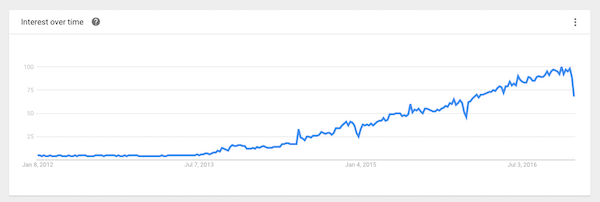
\includegraphics[height=4.2cm]{imagens/docker}
\caption{Gráfico de utilzação do docker entre os anos 2012 e 2016.}
\label{fig:utilizacao-docker}
\end{figure}

A velocidade do micro-serviço permite e incentiva a implementação e estudo dos mesmos. Segundo Adrian (Membro e fundador da eBay Research Labs)  micro-serviços possui características comum, como: Implantação com pouca frequência, novas versões implantadas automaticamente, orquestração de uso geral não é necessário, uma vez que, sistemas inteiros são implantados com todas as partes ao mesmo tempo, arquiteturas utilizam centenas de micro-serviços e cada publicação é altamente customizada.
Seguindo adiante, o próximo passo que Adrian vê é orquestração para aplicações baseadas em padrões portáteis, em vez de dezenas de micro-serviços nas quais novas versões são automaticamente implantadas e que escalabilidade e disponibilidade são asseguradas, prevendo também um movimento contínuo de arquiteturas monolíticas para arquiteturas de micro-serviços. (STENBERG, 2015).

Implantar a Arquitetura de micro-serviços em empresas vai proporcionar diferentes benefícios para a estrutura de negócio como: usufruir de liberdade maior para o desenvolvimento de serviços de modo independente, implantar automaticamente através de ferramentas de integração contínua e código aberto, como Hudson, Jenkins e outras, possibilitar utilização de códigos escritos em linguagens diferentes para diferentes serviços utilizando comunicação REST através de Json ou XML, facilitar a ampliação e integração de micro-serviços com serviços terceirizados, através de APIs, organizar o código em função de capacidades de negócio, dando mais visão das ofertas e necessidades dos clientes. Dentre todos os benefícios citados é possível fazer o gerenciamento otimizado de falhas, o que significa que, se um serviço venha a falhar, os outros continuarão funcionando. Através dos micro-serviços, é possível identificar falhas com mais eficiência, visto que o particionamento favorece uma visão mais detalhada de cada serviço (PELOI, 2016). É possível observar na figura \ref{fig:art-scalability} as três dimensões da escalabilidade, onde o eixo X refere-se à escalabilidade horizontal, para ampliar a capacidade e disponibilidade da aplicação (cada servidor executa uma cópia idêntica do código), Z semelhante à do eixo X,  mas requer a presença de um componente que se responsabilize pelo roteamento das requisições ao servidor adequado, e o eixo Y que representa a terceira dimensão da escalabilidade, denominada decomposição funcional e é responsável por dividir a aplicação em uma série de serviços. A cada serviço corresponde um conjunto de funções (gerenciamento de pedidos, gerenciamento de clientes, entre outros).

\begin{figure}[h]
\centering
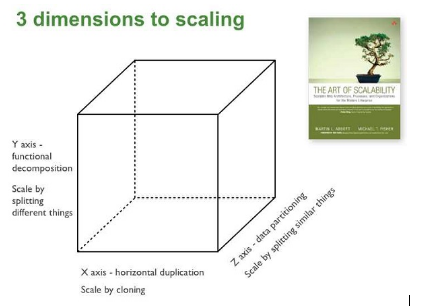
\includegraphics[height=6.2cm]{imagens/scalability}
\caption{The Art of Scalability - 2009.}
\label{fig:art-scalability}
\end{figure}


Segundo dados de Richardson(2014), diversas empresas estão utilizando micro-serviços, dentre as citadas estão: Comcast Cable, Uber, Netflix, Amazon, Ebay, SoundCloud, Karma, Groupon, Hailo, Gilt, Zalando, Lending Club, AutoScout24.
Os problemas associados ao desenvolvimento de software em larga escala ocorreram em torno da década de 1960. Na década de 1970 viu-se um enorme aumento de interesse da comunidade de pesquisa para o design de software em suas aplicações e  no processo de desenvolvimento. Nesta década o design foi muitas vezes considerado como uma atividade não associada com a implementação em si, e portanto requerendo um conjunto especial de notações e ferramentas. Por volta da década de 1980, a integração do design nos processos de desenvolvimento contribuiu para uma fusão parcial dessas duas atividades, tornando assim mais difícil fazer distinções puras.

As referências ao conceito de arquitetura de software também começaram a aparecer década de 1980. No entanto, uma base sólida sobre o tema foi estabelecida apenas em 1992 por Perry Wolf (autor do livro “Foundations for the study of software architecture"). Sua definição de arquitetura de software era distinta do design de software, e desde então tem-se gerado uma grande comunidade de pesquisadores estudando as aplicações práticas da arquitetura de software com base em micro-serviços, permitindo  assim que os conceitos sejam amplamente adotados pela indústria e pela academia.

O advento e a difusão da orientação por objetos, a partir dos anos 80 e, em particular, a década de 1990, trouxe sua própria contribuição para o campo da Arquitetura de Software. O clássico por Gamma et ai. abrange a concepção de software orientado a objetos e como traduzi-lo em código que apresenta uma coleção de soluções recorrentes, chamados padrões. Esta ideia não é nova nem exclusiva à Engenharia de Software, mas o livro é o primeiro compêndio a popularizar a idéia em grande escala. Na era pré-Gamma os padrões para soluções OO já estavam sendo utilizado: um exemplo típico de um padrão de projeto arquitetônico em programação orientada a objetos é o Model-View-Controller (MVC), que tem sido um dos insights seminais no desenvolvimento precoce de interfaces gráficas de usuário.(DRAGONI et al., 2016)

Cerca de sete anos atrás a empresa Netflix (provedora global de filmes e séries de televisão via streaming - distribuição de dados, geralmente de multimídia em uma rede através de pacotes) começou a migrar suas aplicações legadas para uma arquitetura baseada em APIs (Interface de programação de aplicativos) hospedadas na nuvem (local para armazenamento de dados online) da Amazon (empresa transnacional de comércio electrónico dos Estados Unidos com sede em Seattle), influenciando assim, o crescimento de uma ideologia na área de desenvolvimento de softwares que foi batizada pelo nome de “micro-serviço”.

Uma investigação realizada pela empresa Cisco (Companhia sediada em San José, Califórnia, Estados Unidos da América) em 2016 revela que, apesar de toda a euforia sobre a Internet das Coisas, o consumo de de vídeo via internet gera 63\% do tráfego global. A expectativa é que essa marca chegue a 79\% até 2020 e o tráfego de dados gerado por vídeos em resolução Ultra HD subirá de 1.6\% para 20.7\% do total em 2020. Um levantamento realizado pela Cisco VNI Mobile 2016 mostra que os dispositivos IoT mais simples geram uma quantidade de dados equivalentes a 7 veze o que é produzido por um celular comum (não um smartphone). Demandando pouco das redes de telecomunicações, os dispositivos IoT não representarão um grande pessoa para os provedores de infraestrutura na América Latina (IDC, 2016). 

Segundo o relatório “The State of Internet” de 2016, da Akamai (Empresa de Internet americana, sediada em Cambridge, Massachusetts), o país melhor colocado na faixa de redes com banda igual ou maior a 15 Mb/s é o Chile - 4,4\% de seus serviços de Internet atingem essa marca. Entretanto, para chegar a essa posição, o Chile investiu pesadamente entre 2014 e 2015, conseguindo crescer 150\% de um ano para outro. O Uruguai fica logo abaixo, com 4,1\% de sua Internet na faixa dos 15 Mb/s. Atualmente no Brasil, somente 1,1\% dos serviços atingem esta marca.

Na arquitetura de microserviços, se quisermos que um aplicativo seja colocado em esteróides, ele pode ser feito sem afetar outros serviços. Podemos apenas começar a executar este serviço específico em um hardware mais forte. Um microservice único pode ser atualizado nesta arquitetura, sem afetar outros ... a única condição é que o sistema de tempo de execução suporta isso. Cada microservice em uma plataforma pode ser desenvolvido em uma linguagem diferente - Java, C, C ++, Python, etc Governança granular é possível para cada microservice porque não tem dependência em outro. Ele pode ser monitorado e governado separadamente. Essa arquitetura descentraliza o gerenciamento de dados, uma vez que cada microserviço pode armazenar seus dados de uma maneira que se adapte a ele. Arquitetura Microservice suporta automação. É possível mover montagens inteiras de microservices de um ambiente de implementação para outro apenas usando as configurações de perfil com um único clique. Eles são muito mais resistentes do que as aplicações tradicionais. Isto é devido ao fato de que uma única aplicação pode ser retirada de um monte de aplicativos microservices, como estes são independentes uns dos outros.

A arquitetura do microservice tem suas vantagens óbvias e aquela é a razão porque assim que muitos negócios e serviços públicos proeminentes como Netflix, eBay, Amazon, o serviço digital do governo BRIT NICO, realestate.com.au, para diante, Twitter, Paypal, Gilt, Bluemix, Soundcloud , The Guardian, etc, apenas para citar alguns, todos se graduaram de arquitetura monolítica a microservices. Embora este seja o caso, assim como não há um plano perfeito, não há nenhuma arquitetura perfeita. O que funciona sob uma circunstância particular pode se tornar o gargalo em outro.

\subsection{Tecnologias}
Neste trabalho será utilizado no Back-end a tecnologia do netflix Service Discovery (Eureka), e para comunicar com este serviço será utilizado o circuito integrado Nodemcu Esp8266. Existem outras bibliotecas que podem trabalhar em conjunto com o Eureka que são: Circuit Breaker (Hystrix), Intelligent Routing (Zuul) and Client Side Load Balancing (Ribbon). 

\subsubsection{Zuul}
Zuul é a “porta da frente” para todas as requisições de dispositivos e sites para o back-end. O mesmo foi construído para permitir roteamento dinâmico, monitoramento, resiliência e segurança. O Zuul foi desenvolvido pela Netflix pelo fato de que o volume e a diversidade do tráfego da API do mesmo resultam em problemas de produção que surgem rapidamente e  sem aviso prévio, eles precisavam de um sistema que permita os mesmos mudar rapidamente o comportamento e reagir a estas situações.
O Zull utiliza uma variedade de diferentes tipos de filtros que permite-se aplicar rapidamente funcionalidades os serviços de ponta. Esses filtros ajudam a executar as seguintes funções: Autenticação e segurança, identificando requisitos de autenticação para cada recurso e rejeitando solicitações indesejadas. Insights e monitoramento, rastreamento de dados significativos e estatísticas, a fim de dar uma visão precisa da produção. Roteamento dinâmico, encaminhado dinamicamente solicitações para diferentes clusters de backend conforme necessário. Stress Testing, aumento gradual de tráfego para um cluster, a fim de avaliar o desempenho. Load Shedding, alocação de capacidade para cada tipo de solicitação e soltando pedidos que excedem o limite. Manipulação de resposta estática, construção de respostas diretamente na ponta ao invés de encaminhá-las para um cluster interno.
Dentre os vários componentes que integram a biblioteca do Zuul, estão: Zuul-core que contém funcionalidades a fim de compilar e executar filtros, Zuul-simple que mostra como construir um aplicativo com zuul-core, Zuul-netflix que adiciona componentes Netflix utilizando Ribbon para solicitações de roteamento. (Zuul, 2014)

\subsubsection{Ribbon}
Ribbon dá suporte à comunicação entre processos na nuvem e inclui balanceadores de carga desenvolvidos pela netflix. A tecnologia citada fornece os seguintes recursos: regras de balanceamento de carga múltiplas e conectáveis, integração com a descoberta de serviços, resiliência de falhas incorporada, clientes integrados com balanceadores de carga e configuração de clientes utilizando Archaius. O Ribbon é composto pelos seguintes projetos: Ribbon-core que inclui definições de interface e balanceamento de carga e cliente, implementações de balanceador de carga comuns, integração de cliente com balanceadores de carga e fábrica de clientes. Ribbon-eureka que inclui implementações do balanceador de carga com base no Eureka-client (bibliote para registro e descoberta de serviços). Ribbon-httpclient que inclui a inclui a implementação baseada em JSR-311 do cliente REST integrada com balanceadores de carga.

\subsubsection{Hystrix}
Hystrix é um ambiente distribuído, inevitavelmente algumas das muitas dependências de serviços falharão, e esta biblioteca ajuda a controlar as interações entre serviços distribuídos adicionando tolerância de latência e lógica de tolerância a falhas. O mesmo faz isso isolando pontos de acesso entre os serviços, interrompendo falhas em cascata através deles, todas as quais melhoram a resiliência geral do sistema. Atualmente, dezenas de bilhões de threads isoladas e centenas de bilhões não isoladas são executadas utilizando o Hystrix todos os dias na Netflix. Isso resulta em uma melhoria dramática no tempo e atividade e resiliência. Hystrix é projeto para: proteger e controlar a latência e falhas de dependências acessadas por meio de bibliotecas de terceiros, interromper falhas em cascata em um sistema distribuído, recuperação rápida a falhas, monitoramento em tempo real, alertas e controle operacional. Quando se trata de micro-serviços, os mesmos contém dezenas de dependências com outros micro-serviços, o que ocasiona que se um deles falhar e o mesmo não estiver isolado destas falhas externas, corre o risco de também ser afetado. Por exemplo, um aplicativo que dependa de 40 serviços em que cada serviço tem 99,99\% de disponibilidade, pode se esperar: 99,99 \^ 40 = 99,6\% de tempo de atividade, 0.4\% de 1 bilhão de falhas resulta em 4 milhões de falhas. Mesmo que pequena a possibilidade de falha, se somar a quantidade de micro-serviços ao tempo de indisponibilidade que pode surgir por pequenas falhas, o problema pode ser facilmente escalável fazendo com que assim serviços importantes fiquem até mesmos horas indisponíveis. Quando toda a aplicação está funcionando e configurada de maneira correta, o fluxo de solicitações ocorrer conforme a figura \ref{fig:hystrix-overtime}.

\begin{figure}[h]
\centering
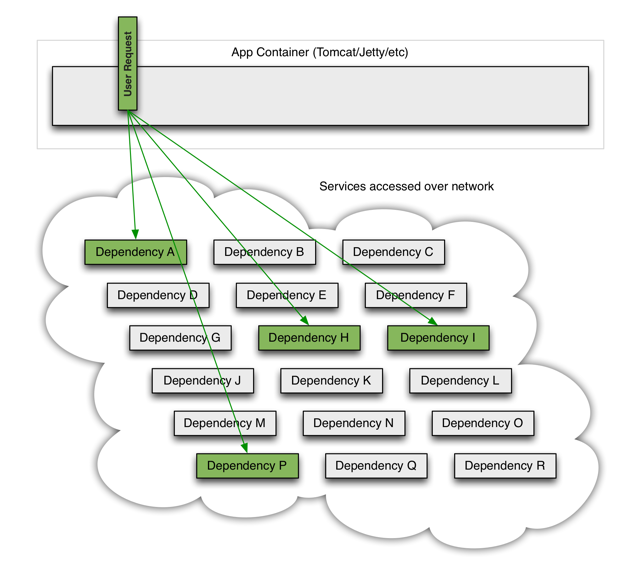
\includegraphics[height=6.2cm]{imagens/figura3}
\caption{Wiki Hystrix (Internet Overtime) - 2015).}
\label{fig:hystrix-overtime}
\end{figure}

Quando um dos muitos serviços se torna latente, ele pode bloquear toda a solicitação do usuário, conforme apresentado na figura \ref{fig:hystrix-dimensions-scaling}.

\begin{figure}[h]
\centering
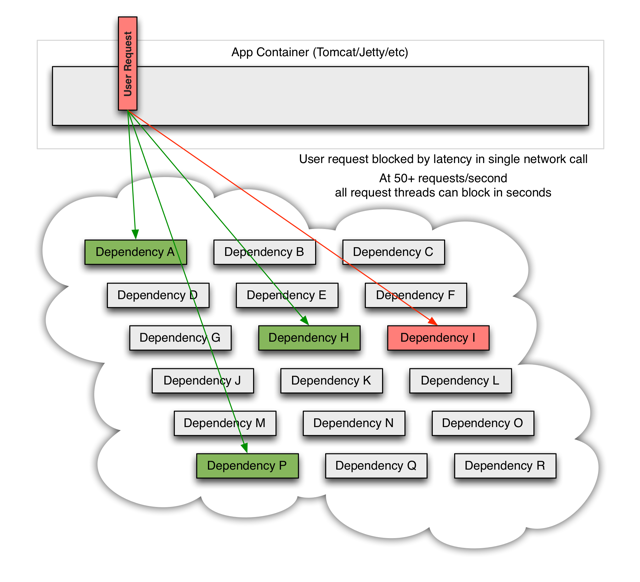
\includegraphics[height=6.2cm]{imagens/figura4}
\caption{Wiki Hystrix (3 dimensions to scaling) - 2015).}
\label{fig:hystrix-dimensions-scaling}
\end{figure}

Com tráfego de alto volume, uma única dependência com latência excessiva, pode fazer com todos os recursos fiquem saturados em segundo. Cada ponto em um aplicativo que atinge a rede ou em uma biblioteca cliente que pode resultar em solicitações de rede é uma fonte de falha potencial. Pior que falhas, esses aplicativos também podem resultar em latências aumentadas entre os serviços, que faz backup de filas e outros recursos do sistema, causando ainda mais falhas em cascata em todo a aplicação, conforme a figura \ref{fig:hystrix-container}.

\begin{figure}[h]
\centering
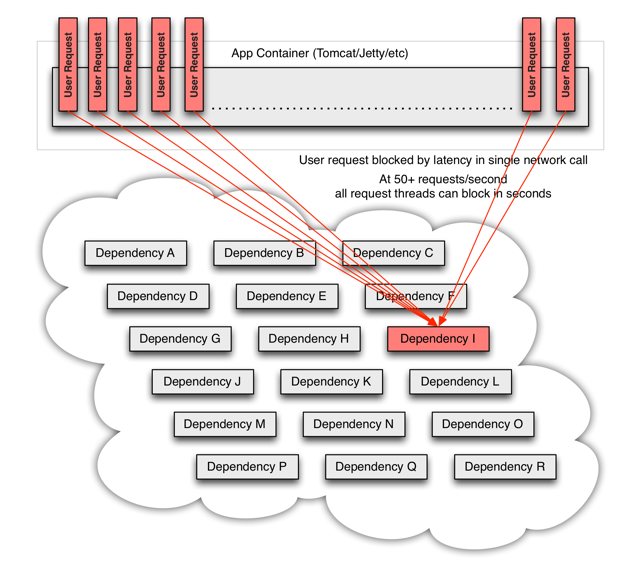
\includegraphics[height=6.2cm]{imagens/figura5}
\caption{Wiki Hystrix (Container) - 2015).}
\label{fig:hystrix-container}
\end{figure}

A biblioteca Hystrix subjaz os seguintes princípios de design: Impedir que qualquer dependência única utilize todos as threads de usuários de container (como Tomcat), desperdiçando carga, fornecer soluções sempre que possível para proteger os usuários contra falhas, utilizando técnicas de isolamento para limitar o impacto de qualquer dependência, otimizar o tempo de descoberta através de métricas, monitoramento e alertas em tempo quase real, otimizando o tempo de recuperação por meio de propagação de baixa latência de alterações de configuração e suporte para alterações de propriedade dinâmicas na maioria dos aspectos do Hystrix, o que permite fazer modificações operacionais em tempo real com loops de realimentação de baixa latência, protegendo contra falhas em toda a execução do cliente de dependência, não apenas no tráfego da rede. (Hystrix, 2015)

\subsubsection{Eureka + Spring Cloud}
Spring Cloud fornece integrações Netflix OSS para Spring Boot por meio de auto-configuração e vinculação ao Spring Environment e outros padrões de programação Spring. Dentre os produtos spring Cloud encontra-se os clientes Eureka ou Service Discovery que é um dos princípios fundamentais de uma arquitetura baseada em micro-serviços. Configurar um micro-serviço é trabalhado pois envolve diversas técnicas de descoberta e registro de serviços, e com o Service Discovery da Netflix torna-se eficiente este trabalho pois com poucas anotações Java consegue-se criar uma aplicação simples Eureka. 

Eureka também vem com um componente de cliente baseado em Java, o cliente Eureka, que torna as interações com o serviço muito mais fácil. Ocliente também tem um balanceador de carga incorporado que faz balanceamento de carga round-robin (Algoritmos simples de agendamento e escalonamento de processos) básico. Quando um cliente se registra no mesmo, o mesmo fornece metadados sobre, como host e porta, dentre outras informações que podem ser encontradas na documentação. Se o registro falhar durante a configuração, a instância da aplicação é removida do registro. Em resumo, o Eureka é um serviço baseado em REST (Representational State Transfer) que é utilizado principalmente na AWS (Amazon Web Services) para localizar serviços com a finalidade de balanceamento de carga e failover (tolerância a falhas) de servidores de camada intermediária. 

A Amazon possui um produto chamado AWS ELB (Amazon Web Services Elastic Load Balancer), que é uma solução de balanceamento de carga para serviços de ponta expostos ao tráfego web do usuário final, e a diferença entre o mesmo e o produto da Netflix, é que o Eureka preenche a necessidade de balanceamento de carga médio. Embora teoricamente pode-se colocar serviços de nível intermediário atrás do AWS ELB, no EC2 classic (Elastic Compute Cloud) pode-se expor ao mundo exterior e perder toda a utilidade dos grupos de segurança AWS. O AWS ELB  também possui uma solução de balanceamento de carga em proxy (servidor intermediário para requisições entre cliente e servidor final) tradicional, enquanto no Eureka, o balanceamento ocorre no nível da instância, servidor e host. As instâncias do cliente sabem todas as informações sobre quais aplicações precisam conversar.

Uma questão a ser analisada no Eureka, é o DNS (Domain Name System). Dentre as aplicações existente para resolução de DNS está o Route 53, um serviço de nomeação, como o qual Eureka pode fornecer o mesmo para os servidores de nível médio. Route 53 é um serviço DNS e também pode fazer roteamento baseado em latência em regiões AWS. Eureka é análogo ao DNS interno e não tem nada a ver com os servidores DNS em todo o mundo. Eureka também é isolado no sentido de que não sabe sobre servidores em outras regiões AWS. Sua finalidade principal de manter informações é para balanceamento de carga dentro de uma região.

Na Netflix, além de desempenhar um papel crítico no balanceamento de carga de nível médio, o Eureka é utilizado para os seguintes fins: implementações com Netflix Asgard, um serviço para fazer atualizações de serviços de forma rápida e segura, registro e exclusão de instâncias e transporte de metadados específicos de aplicativos adicionais sobre serviços. Dentre os motivos para utilizar o Eureka está o fato que o mesmo provê uma solução para balanceamento de carga round-robin simples, e quem não estiver disposto a se registrar com o AWS ELB e expor seu tráfego externamente, o mesmo resolve este problema.

Com o Eureka, a comunicação é transparente, pois o mesmo fornece informações sobre os serviços desejados para comunicação, mas não impõe quaisquer restrições sobre o protocolo ou método de comunicação. Exemplificando, pode-se utilizar o Eureka para obter o endereço do servidor destino e utilizar protocolos como thrift, http (s) ou qualquer outro mecanismos RPC (Remote Procedure Call) que permite fazer conexões ou chamadas por espaço de endereçamento de rede. 

\subsubsection{Modelo Arquitetural Eureka}
O modelo arquitetural implantado na Netflix utilizando o Eureka é  descrita na figura \ref{fig:wiki-eureka-est}. Existe um cluster por região que conhece somente instâncias de sua região. Há pelo menos um servidor Eureka por zona para lidar com falhas da mesma. Os serviços se registram e, em seguida, a cada 30 segundos enviam os chamados “batimentos cardíacos” ou requisições para renovar seus registros. Se o cliente não renovar o registro, ele é retirado do servidor em cerca de 90 segundos. As informações de registro e renovações são replicadas para todos as conexões no cluster. Os clientes de qualquer zona podem procurar as informações do registro para localizar seus serviços que podem estar em qualquer zona e fazer chamadas remotas.

Para serviços não baseados em Java, tem-se a opção de implementar a parte do cliente utilizando o protocolo REST desenvolvido para o Eureka ou executar um “side car” que é uma aplicação Java com um cliente embutido Eureka que manipula os registros e conexões. Quando se trabalha com serviços em nuvem, pensar em resiliência se torna ímprobo. Eureka se beneficia dessa experiência adquirida, e é construído para lidar com falha de um ou mais servidores do mesmo.

\begin{figure}[h]
\centering
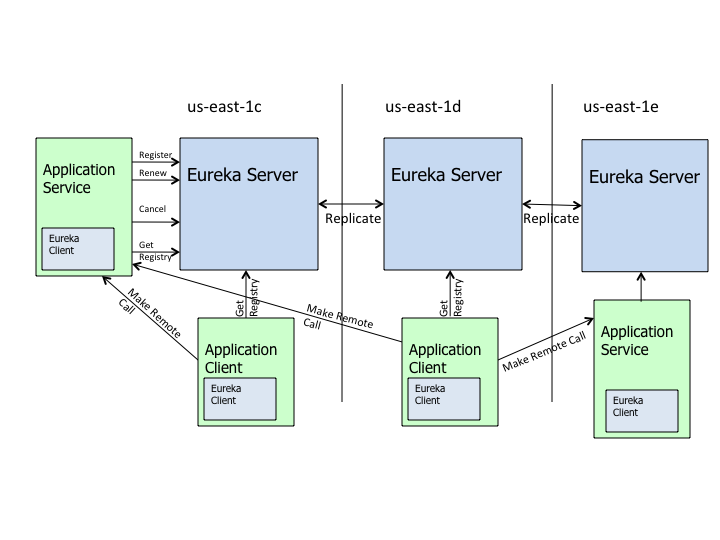
\includegraphics[height=6.2cm]{imagens/figura6}
\caption{Wiki Eureka - 2015).}
\label{fig:wiki-eureka-est}
\end{figure}







% Exemplo tabela
% \begin{table}[h]
% \centering
% \caption{ Modelo de como as tabelas devem ser inseridas no texto }
% \vspace{0.2in}
% \newcolumntype{C}{>{\centering\arraybackslash}X}%
% \newcommand{\rowstyle}[1]{%
%   \protected\gdef\currentrowstyle{#1}%
% }
% \begin{tabularx}{\textwidth}{>{\bf}C|C|C|C}
% \hline 
% \textbf {Índice} & \textbf{Coluna 01} &\textbf{ Coluna 02} & \textbf{Coluna 03} \\ \hline \hline
% Linha 01 & & & \\ \hline
% Linha 02 & & & \\ \hline                         

% \end{tabularx}
% \end{table}
